\documentclass{article}
\usepackage[utf8]{inputenc}
\usepackage[spanish]{babel}
\usepackage{amsmath}
\usepackage{multicol}
\usepackage{graphicx}
\usepackage{float}
\usepackage{geometry}
\usepackage{listings}
\usepackage{enumitem}

\title{Report of the model SIRSV}
\author{PropEnfermedades APP}
\date{}
\geometry{letterpaper, top=2.54cm, bottom=2.54cm, left=3cm, right=3cm}    
\setlength{\parindent}{0cm}
\setlength{\parskip}{0.2em}

\begin{document}
\maketitle
\section{Model}
Next we show the model used in the simulation.
\subsection*{Description}
SIRSV model, which represents the spread of an infectious disease in a population considering births and deaths, in addition to vaccination.
\subsection*{Equations}
\begin{equation}
\begin{split}
S' = -(b * S * I) - (m * S) + (m * N) - (g1 * (m * N)) - (g2 * S) \\ I' = (b * S * I) - (v * I) - (m * I) \\ R' = (v * I) - (m * R) + g1 * (m * N)
\end{split}
\end{equation}
\subsection*{Parameters}
\begin{itemize}
\item $m = 0.06$. 
\item $b = 0.5$. 
\item $v = 0.2$. 
\item $g_1 = 0.05$. 
\item $g_2 = 0.04$. 
\end{itemize}
\subsection*{Initial values}
The initial values used in the simulation are (The values are normalized respect to 7900000 that is the total population):
\begin{itemize}
\item $S_0 = 0.999999$. 
\item $I_0 = 1.26582e-06$. 
\item $R_0 = 0$. 
\item $t_0 = 0$. 
\item $t_f = 150$. 
\item $dt = 0.5$. 
\end{itemize}
\section*{Results}
The maximum infected population is 3534.37 is reached on day 149.5.
Next we show the results of the simulation using the model SIRSV with the parameters and initial values shown above.
\begin{figure}[H]
\centering
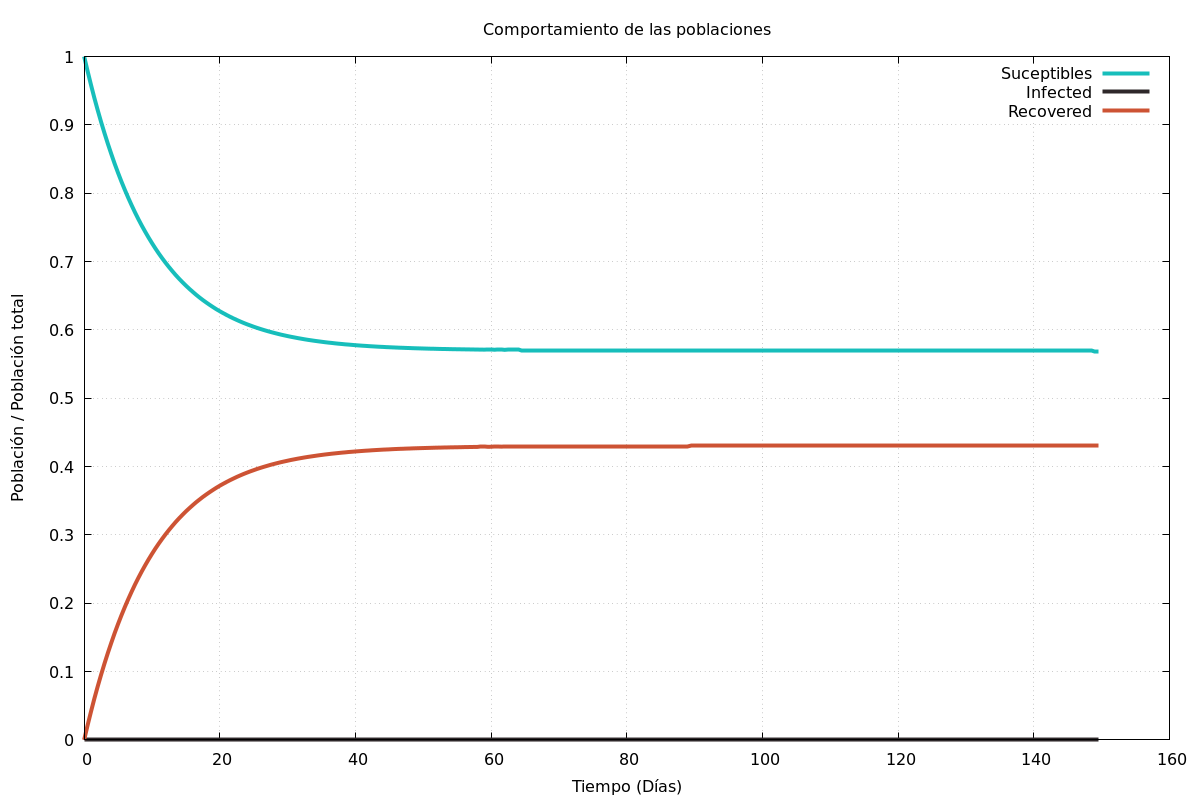
\includegraphics[width=0.8\textwidth]{./data/PryectoSIRSVAC/graph-SIRSV.png}
\caption{Graph of the model SIRSV}
\end{figure}
\begin{figure}[H]
\centering
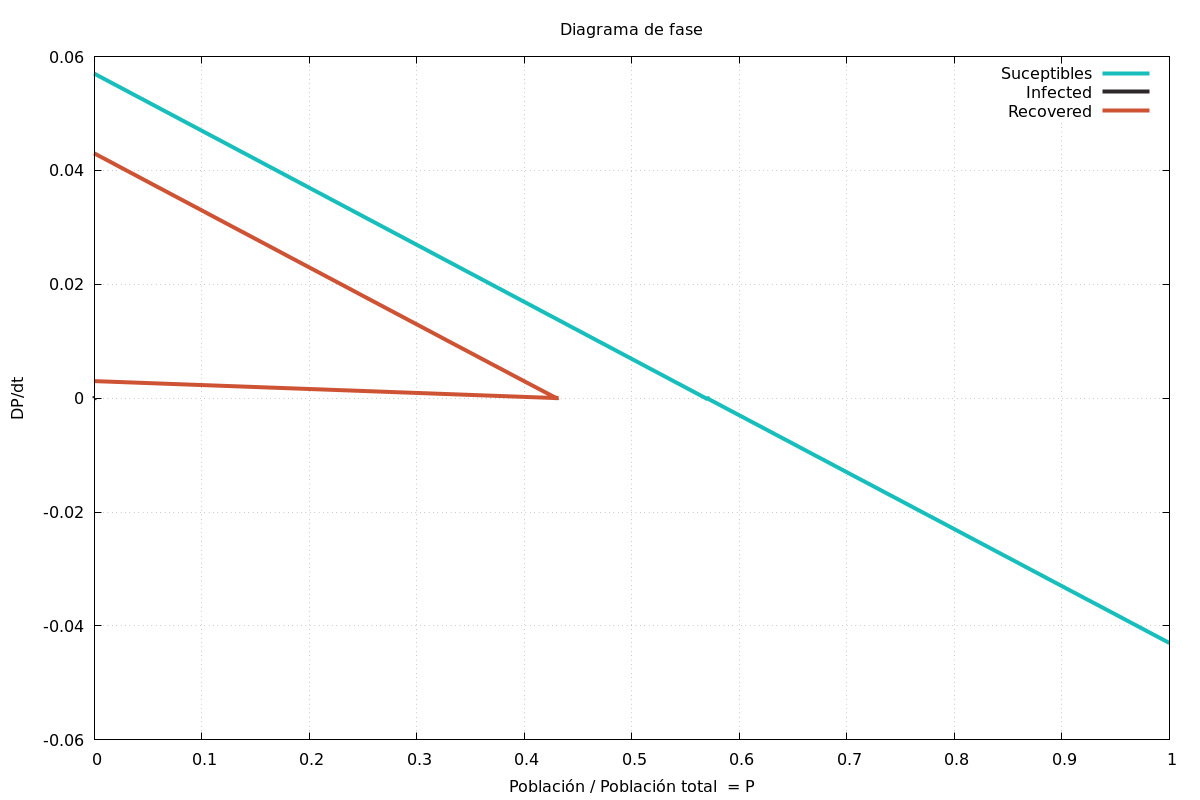
\includegraphics[width=0.8\textwidth]{./data/PryectoSIRSVAC/phase-SIRSV.png}
\caption{Phase portrait of the model SIRSV}
\end{figure}
\end{document}
